\documentclass[a4paper]{article}
\renewcommand{\rmdefault}{ftm}
\usepackage{graphicx}
\usepackage[14pt]{extsizes}
\usepackage[utf8]{inputenc}
\usepackage[russian]{babel}
\usepackage{setspace,amsmath}
\usepackage[left=25mm, top=15mm, right=10mm, bottom=25mm, nohead, footskip=10mm]{geometry}
\begin{document}
\begin{center}
\hfill \break
\large{\textbf{ФГБОУ ВО«Московский Политехнический университет»}}\\
\hfill \break
\hfill \break
\hfill \break
\hfill \break
\hfill \break
\hfill \break
\hfill \break
\large{Лабораторная работа№8}\\
\footnotesize{Программрование в графчиеском режиме\\
Задание 1\hspace{3cm}Вариант№7\break\\
По дисциплине:\\
Основы Программирования
}
\end{center}
\hfill \break
\hfill \break
\hfill \break
\hfill \break
\hfill \break
\hfill \break
\hfill \break
\hfill \break
\hfill \break
\hfill \break
\normalsize{ 
\begin{tabular}{ccc}
\hspace{4cm}Выполнил & Шукуров Ф.Ф  & группа 181-362\\
\\
\hspace{4cm}Проверил & \underline{\hspace{3cm}}& Никишина И.Н
\end{tabular}
}
\hfill \break
\hfill \break
\hfill \break
\hfill \break
\hfill \break
\hfill \break
\hfill \break
\hfill \break
\hfill \break
\hfill \break
\hfill \break
\hfill \break
\begin{center}\texttt{Москва 2018}\end{center}
\thispagestyle{empty}

\newpage
Лабораторная работа№8;
\\
    \begin{lab1}
        \begin{center}\underline{\hspace{6cm}}\\
            Задание:
        \end{center}
        1) Нарисовать график для занного ряда тейлора:\\
        y(x) = -$\frac{\pi}{2}$+$\displaystyle\sum_{n-0}^{\infty}\frac{(-1)^n^+^1}{(2\cdot n+1)\cdot x^2^\cdot ^n^+^1} = -\frac{\pi}{2} - \frac{1}{x}+\frac{1}{3\cdot x^3} - \frac{1}{5\cdot x^5}\dots,\hspace{1cm} x<-1$\\
        2) Для триганометрического выражения:\\
        z(x) = arctgx+b.\\
        где b ~-- введенный пользователем коэффициент смещения графика.
    \begin{description}
        Описание программы:\\
        \small{Программа была написанна на python 3.6, реализованна в среде os Linux, отвечает за ввод данных, вычисление и вывод данных на экран в виде графика.}
    \end{description}
    \begin{algoritm}
        Описание Алгоритма:
        \small\begin{enumerate}
            \item 
                Импортируем необходимые фукнции, в том числе и ранее установленный модуль matplotlib
            \item
                Создаем проверку пользовательского ввода в диапазоне от -$\infty$ до -1 в иницилизированном ранее бесконечно цикле.
            \begin{enumerate}
                \item 
                    Используя блок исключений (if$\to$elif$\to$else), в случае <<Истины>>, выход из цикла
                \item 
                    Присваиваем пользовательский ввод к float значению.
            \end{enumerate}
            \item 
                Присваиваем dx пользовательский ввод с клавиатуры
            \item 
                Создавая два пустых массива, так же инициализируем, цикл с условием <<xEnd$\leq$xt>>
            \item 
                Используя алгоритм работы (см.Лабораторная работа№3, задание№3) вычисления значений ряда Тейлора, добавляем результат вычсилений к coo\_y ~-- координаты y, и <<xt>>, к coo\_x ~-- координаты x.
            \begin{enumerate}
                \item 
                    После вычислений, аннулям результат, для корректных вычислений.
            \end{enumerate}
            \item 
                С помощью matplotlib.pyplot(далее plt).plot(\underline{\hspace{10mm}}, передаем массив координат по <<X>> и <<Y>>, указываем необходимый цвет.
            \item 
                С помощью numpy.linspace(xBeg, xEnd, num = 100), добавялем в промежутках между числами до 100 элементов, для более плавного графика <<x>>
            \item 
                Используя numpy.arctan(x) + b, где b ~-- смещение графика по y.
        \end{enumerate}
    \end{algoritm}
        \texttt{Листинг Программы:}
    \begin{verbatim}
import numpy as np
import matplotlib.pyplot as plt
while True:
    while True:
        xBeg = float(input("xBeg(-"+u"\u221E"+":-1)= "))
        if xBeg<-1:
            break
    xEnd = float(input("xEnd()-"+u"\u221E"+":-1) = "))
    if xEnd<-1:
        break
dx = float(input("dx = "))
xt=xBeg
coo_x, coo_y = [], []
while xt>=xEnd:
    n=0
    result_1 = 0
    result_1 = ((-1)**(n+1))/(((2*n)+1)*(xt**((2*n)+1)))
    coo_x.append(xt)
    coo_y.append(-np.pi/2+result_1)
    xt-=abs(dx)
    result_1 = 0
b = int(input("B = "))
x = np.linspace(xBeg, xEnd, num=100, endpoint=False)
plt.plot(coo_x,coo_y,color = "#0349e8")
plt.plot(x, np.arctan(x)+b, color = "green")
plt.axis('tight')
plt.ylabel('Y')
plt.title('X')
plt.show()
    \end{verbatim}
    \begin{center}
        Результат работы программы:
    \end{center}
    \begin{verbatim}
xBeg(-∞:-1)= -10
xEnd()-∞:-1) = -100
dx = 0.1 
B = 1
    \end{verbatim}
    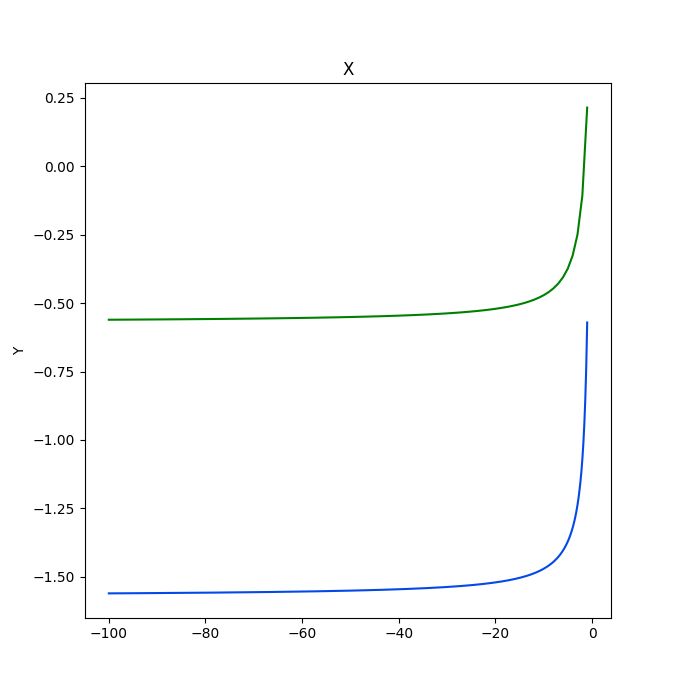
\includegraphics[width=100mm,scale=0.5]{Figure_1.png}
    \end{lab1}    
    
\end{document}
